\documentclass{article}
\usepackage{tikz}
\usepackage{amsmath}
\usetikzlibrary{decorations.markings}

\begin{document}

\begin{center}
\Large\textbf{Beautiful Mathematical Patterns}
\end{center}

\section*{The Golden Spiral and Fibonacci Rectangles}
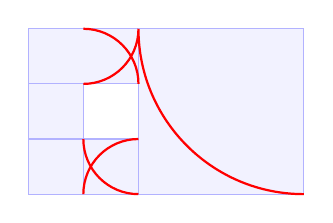
\begin{tikzpicture}[scale=0.7]
    % Fibonacci rectangles
    \draw[blue!30, fill=blue!5] (0,0) rectangle (1,1);
    \draw[blue!30, fill=blue!5] (1,0) rectangle (2,1);
    \draw[blue!30, fill=blue!5] (0,1) rectangle (1,2);
    \draw[blue!30, fill=blue!5] (0,2) rectangle (2,3);
    \draw[blue!30, fill=blue!5] (2,0) rectangle (5,3);
    
    % Golden spiral
    \draw[thick, red] (1,1) arc (180:270:1)
        (2,1) arc (90:180:1)
        (2,2) arc (0:90:1)
        (1,2) arc (-90:0:1)
        (2,3) arc (180:270:3);
\end{tikzpicture}

\section*{Wave Patterns}
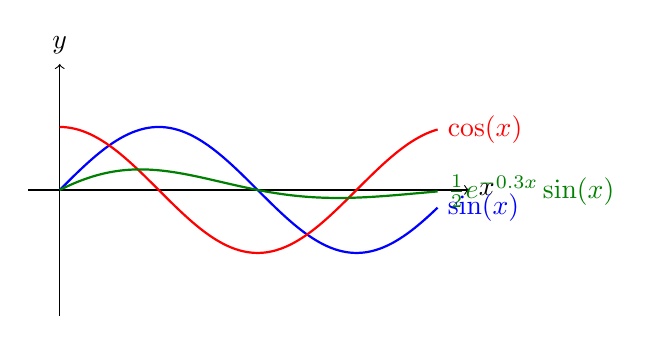
\begin{tikzpicture}[scale=0.8]
    % Axes
    \draw[->] (-0.5,0) -- (6.5,0) node[right] {$x$};
    \draw[->] (0,-2) -- (0,2) node[above] {$y$};
    
    % Functions
    \draw[blue, thick, domain=0:6, samples=100] 
        plot (\x,{sin(\x r)}) node[right] {$\sin(x)$};
    \draw[red, thick, domain=0:6, samples=100] 
        plot (\x,{cos(\x r)}) node[right] {$\cos(x)$};
    \draw[green!50!black, thick, domain=0:6, samples=100] 
        plot (\x,{0.5*exp(-0.3*\x)*sin(\x r)}) node[right] {$\frac{1}{2}e^{-0.3x}\sin(x)$};
\end{tikzpicture}

\section*{Sunflower Pattern}
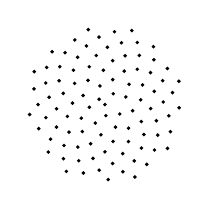
\begin{tikzpicture}
    % Generate points using golden angle (≈ 137.5°)
    \foreach \n in {0,...,100}{
        \node[circle, fill, inner sep=0.5pt] at 
            ({0.1*sqrt(\n)*cos(\n*137.5)}, 
             {0.1*sqrt(\n)*sin(\n*137.5)}) {};
    }
\end{tikzpicture}

\end{document}